\documentclass{article}
\usepackage{amsmath}
\usepackage{amssymb}
\usepackage{graphicx}
\usepackage{kotex}
\author{lichen}
\date{\today}
\title{culture media design by DoE}
\newcommand{\imp}[1]{\textbf{\textit{#1}}} 
\begin{document}
\begin{titlepage}
    \maketitle
\end{titlepage}

\section{Bioprocess Optimization Using Design-of-Experiments Methodology\cite{mandenius2008bioprocess}}

\subsection{in vitro experiment process}
실험에 중요한 요소를 경험적으로 추론, 각 요소의 범위를 결정.\\
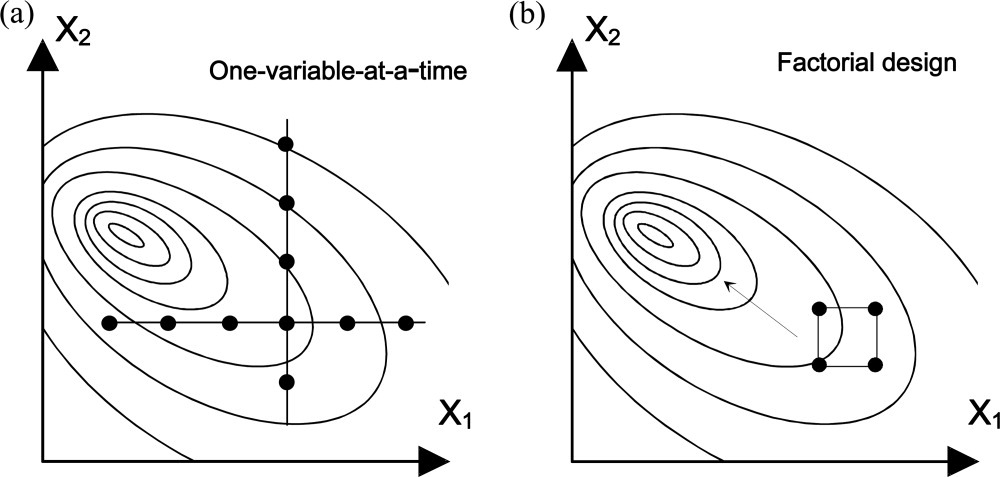
\includegraphics[scale=0.3]{surface.jpg}\\
한번에 한 요소를 바꾸는 실험의 경우 실험 결과가 최적에 도달하기 까지 많은 시행 필요하기 때문에 여러 요소의 조합을 중복없이 시험하여 모델을 설정하고 검증함. 이러한 실험방법을 Factorial Design이라고 함.\\
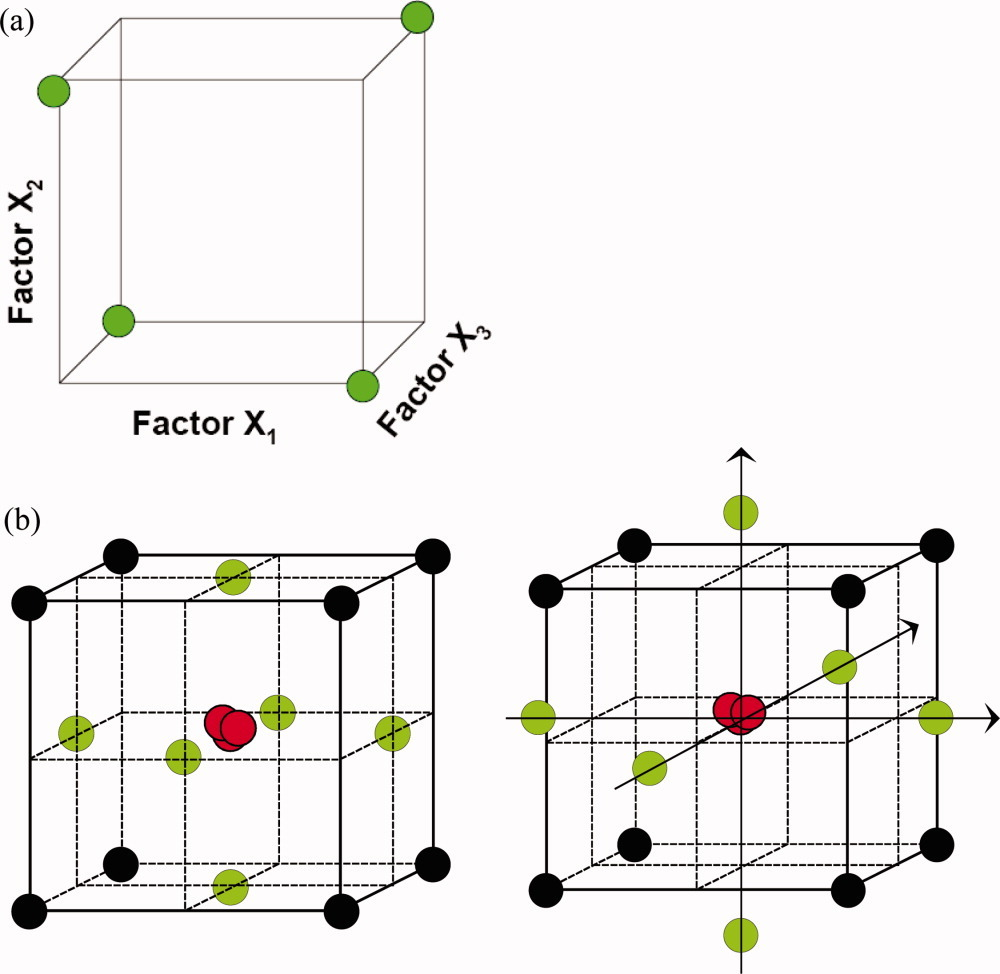
\includegraphics[scale=0.2]{fatorial design.jpg}\\
2 수준 실험에선는 가능한 모든 경우의 수를 시험해 볼 수도 있지만, 요소의 수가 많아지면 그 중 일부만 실험하게 됨. 다변수 실험의 경우 한 중앙값을 잡아 반복 실험을 진행함. 또한 실험 진행에서 오류를 막기 위해 실험 순서를 무작위로 배열 $\rightarrow$ 일반적인 소프트웨어는 실험에 사용하는 요소와 상관관계를 입력하면 실험에 사용할 요소의 조합과 수준, 반복 횟수를 제시함.
\subsection{experimental data explain}
소프트웨어(Matlab, SPSS, MiniTab, JMP, python, R등)를 통해 목표로 하는 값(세포 성장 속도, 대사 작용 등)을 분석
\subsection{data procssing}
\textbf{MLR, Multiple Linear Regression}, \textbf{PLS, Partial Least Squares} 사용,
모델의 적합성과 예측 가능성을 $R^2,Q^2$ 지표로 계산 DoE를 통한 FD를 진행하면 모델의 최적 값뿐만 아니라 모델의 안정성을 확인 할 수 있음 (Taguchi method)
\subsection{results}
FD를 \textit{Pachysolen tannophilus}의 성장을 최적화하기 위해 적용하여 2개의 요소 (온도,PH) 수준에 따라 실험을 19번(9개 조건에서 두 번 반복하여)진행하고 반응 표면을 작성하여 최적의 성장조건을 탐색함.\\
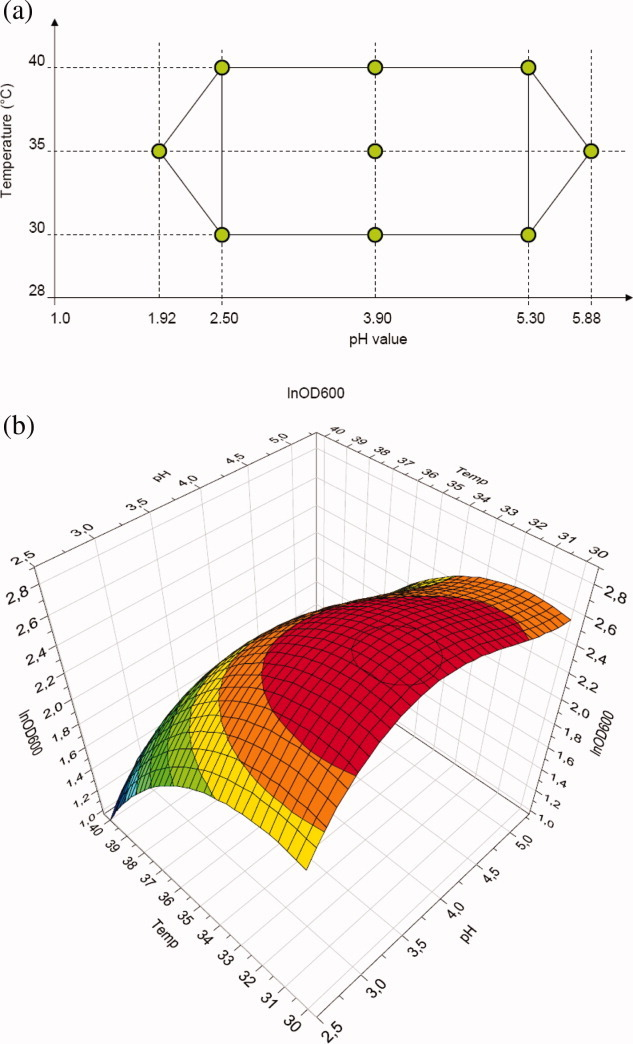
\includegraphics[scale=0.3]{fd.jpg}
\newpage
\section{Evaluation and optimization of hepatocyte culture media
factors by design of experiments (DoE) methodology\cite{dong2008evaluation}}
human hepatoma cell line, C3A을 위한 배지 최적화 \\
목표 : hepatoma cell의 대사 작용에 대해 배지를 최적화 하는 것\\
$\rightarrow$ HGF, OSM, FGF4, EGF, albumin, nicotin-
amide, dexamethasone의 요소가 Urea, Lac, LDH 반응에 미치는 영향 조사
\subsection{in vitro experiment process}
\begin{itemize}
    \item Cell materials and culture procedures
    \item Analytical methods : enzymatic test kits 사용하여 6일에 걸쳐 2일 마다 대사 물질 수준 측정
\end{itemize}
Modde 사용하여 \textbf{two-level factioral design}실험 설계, 7개 요소에 대해 3개의 수준씩 실험진행 
\begin{center}
    \begin{tabular}{||c | c c c c c c c | c c c||} 
     \hline
     Exp.no&  HSA & HGF & OSM  &DexM&  FGF4 & EGF & NicA  &Urea  &  Lac  &  LDH\\
     \hline\hline
     1&0&0&0&7.4&50&100&10&6.3&133.0&35.0\\
     2&6&0&0&0.0&0&100&100&9.0&135.0&147.0\\
     3&0&50&0&0.0&50&0&100&7.6&110.0&22.3\\
     4&6&50&0&7.4&0&0&10&6.3&149.0&23.0\\
     5&0&0&50&7.4&0&0&100&8.0&132.0&8.0\\
     6&6&0&50&0.0&50&0&10&9.6&143.0&27.6\\
     7&0&50&50&0.0&0&100&10&8.0&137.0&27.0\\
     8&6&50&50&7.4&50&100&100&6.3&87.0&25.7\\
     9&3&25&25&3.7&25&50&55&6.7&147.0&24.7\\
     10&3&25&25&3.7&25&50&55&8.0&149.0&22.7\\
     11&3&25&25&3.7&25&50&55&8.3&139.0&30.0\\
     \hline
    \end{tabular}
\end{center}
실험 결과를 통해 주요 요소를 선별하고 주요 요소를 중심으로 추가 실험 진행 
\begin{center}
    \begin{tabular}{||c | c c c c | c c c||} 
     \hline
     Exp.no.&HGF&OSM&FGF4&Urea&Lac&LDH&Alb\\
     \hline\hline
1&0&0&0&8.0&121&34.0&14.1\\
2&40&0&0&11.0&123&44.0&12.0\\
3&0&50&0&14.0&202&66.0&18.4\\
4&40&50&0&14.0&135&86.0&7.13\\
5&0&0&40&7.0&76.6&28.0&17.8\\
6&40&0&40&8.0&134&21.0&9.8\\
7&0&50&40&11.0&177&44.0&9.2\\
8&40&50&40&14.0&130&127&2.6\\
9&0&25&20&10.0&176&42.0&7.0\\
10&40&25&20&13.0&140&95.0&5.3\\
11&20&0&20&9.0&139&28.0&14.6\\
12&20&50&20&9.0&185&43.0&5.8\\
13&20&25&0&12.0&180&60.0&4.9\\
14&20&25&40&9.0&186&47.0&4.9\\
15&20&25&20&14.0&132&74.0&6.9\\
16&20&25&20&10.0&191&51.0&4.7\\
17&20&25&20&11.0&175&50.0&6.0\\
18&0&0&0&8.0&123&32.0&18.3\\
     \hline
    \end{tabular}
\end{center}
\subsection{experimental data explain}
\subsection{data procssing}
\begin{itemize}
    \item model parameter select : 분산을 측정하여 결과 값에 가장 영향력 있는 요소를 측정\\ 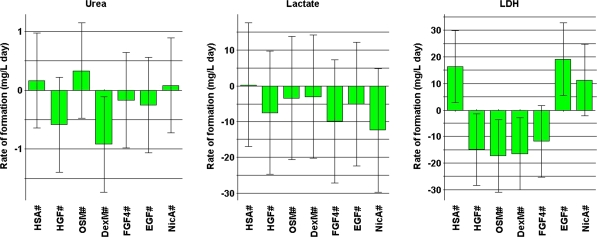
\includegraphics[scale=0.5]{variance.jpg}
    \item reaction surface : 동일한 수준의 결과를 얻는 요소의 조합을 통해 경제적으로 우수한 조건을 탐색할 수 있음\\ 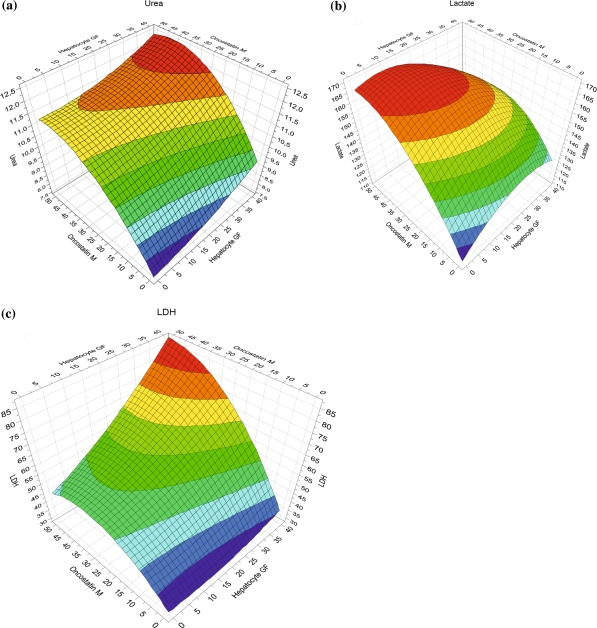
\includegraphics[scale=0.3]{reactionsurfae.jpg}
\end{itemize}
\subsection{results}
\begin{itemize}
    \item hepatocyte growth factor, oncostatin M, and fibro-blast growth factor 4 significantly influenced the metabolic activities of the C3A cell line
    \item hepatocyte growth factor 30 ng/ml, oncostatin 35 ng/ml is optimal level for meida
\end{itemize}
\bibliographystyle{plain}
\bibliography{1}    
\end{document}